% =====================================================================
%  Draft for IEEE Transactions (TIE / TTE / TDE style)
%  Adaptive RCESO for PMSM drives under misalignment-induced periodic load
%  Compiler: pdflatex (two passes)
%  NOTE: [TO BE FILLED] boxes mark every place that needs bench data.
% =====================================================================
\documentclass[journal]{IEEEtran}
\usepackage{cite}
\usepackage{amsmath,amssymb,amsthm,mathtools}
\usepackage{array,booktabs}
\usepackage{graphicx}
\usepackage{xcolor}
\usepackage{tikz}
\usetikzlibrary{positioning,arrows.meta}
\usepackage{balance}
\usepackage[hidelinks]{hyperref}
\allowdisplaybreaks
\interdisplaylinepenalty=2500
\renewcommand{\topfraction}{0.92}
\renewcommand{\textfraction}{0.08}
\renewcommand{\floatpagefraction}{0.8}
\renewcommand{\dbltopfraction}{0.9}
\pdfstringdefDisableCommands{\def\IEEEmembership#1{}}

\newtheorem{lemma}{Lemma}
\newtheorem{theorem}{Theorem}
\newtheorem{proposition}{Proposition}
\newtheorem{corollary}{Corollary}
\theoremstyle{remark}
\newtheorem{remark}{Remark}

\newcommand{\ef}{e_f}
\newcommand{\st}{\operatorname{tanh}}
\newcommand{\ath}{\operatorname{tanh}^{-1}}
\newcommand{\qq}[1]{\textquotedblleft#1\textquotedblright}
\newcommand{\PH}[1]{\par\smallskip\noindent{\color{red!70!black}\fbox{\parbox{\dimexpr\linewidth-2\fboxsep-2\fboxrule}{\footnotesize\textbf{[TO BE FILLED]}\ #1}}}\par\smallskip}
\newcommand{\TODO}[1]{\textcolor{red!70!black}{\footnotesize[TODO: #1]}}

\begin{document}

\title{Repetitive-Control-Enhanced ESO With Proportional-Gain Scheduling and
Event-Triggered Memory Reset for PMSM Drives Under Misalignment-Induced
Periodic Load Torque}

\author{First~A.~Author,~\IEEEmembership{Member,~IEEE,}
        and~Second~B.~Author,~\IEEEmembership{Senior~Member,~IEEE}
\thanks{Manuscript received Month XX, 2026; revised Month XX, 2026.
This work was supported by [funding agency, grant no.]. (Corresponding author: X.)}
\thanks{F.~A.~Author is with [Department], [University], [City], [Country] (e-mail: xxx@xxx.edu).}
\thanks{S.~B.~Author is with [Department], [University], [City], [Country].}}

\markboth{IEEE Transactions on Industrial Electronics, Vol.~XX, No.~X, 2026}%
{Author \MakeLowercase{\textit{et al.}}: Adaptive RCESO for PMSM Drives Under Misalignment}

\maketitle

\begin{abstract}
Misalignment in permanent-magnet synchronous motor (PMSM) drive trains modulates
the load torque at the shaft rotational frequency and its harmonics, injecting a
narrow-band periodic disturbance that a bandwidth-limited extended state observer
(ESO) cannot follow. A low-pass repetitive-control-enhanced ESO (RCESO) provides
the missing internal model, but two problems remain unsolved in the literature:
the large speed dip during a load step, and the echo produced when the internal
model replays a memory that is no longer valid after a disturbance event. This paper
addresses both. First, a gray-box RCESO is formulated in which the ESO and the
low-pass repetitive channel are coupled through a single tracking error, and a
uniform ultimate boundedness (UUB) proof is given, including the effect of gain
scheduling. Second, a proportional-gain scheduling law (Law~D) is driven by the
$T$-window mean of the tracking error, a detector that is structurally blind to
$k\cdot f_0$ components and therefore picks out non-periodic events for free; a
$2^2$ full-factorial ablation shows that Law~D is the factor carrying the Pareto
improvement over all seven evaluation windows, reducing the load-transient RMS error
from 66.80 to 48.36~rpm ($-27.6\%$) without increasing peak current. Third, an event-triggered
state-reset law (Law~F) is derived with two implementations: feedforward (F-A,
event signal available) and envelope-detected (F-B). A timing law shows that the
attainable echo suppression is a monotone function of the detection lag; F-A cuts the
first-cycle echo from 127.7 to 32.5~rpm at a steady-state cost of 0.2\%, whereas F-B
achieves 88.9~rpm at 4.3\%.
Simulation and [TO BE FILLED: experimental] results on a 200~W PMSM test bench
confirm the analysis.
\end{abstract}

\begin{IEEEkeywords}
Active disturbance rejection control (ADRC), extended state observer (ESO),
repetitive control, permanent-magnet synchronous motor (PMSM), misalignment,
periodic disturbance rejection, gain scheduling, event-triggered reset,
uniform ultimate boundedness (UUB).
\end{IEEEkeywords}

\section{Introduction}
\IEEEPARstart{P}{eriodic} torque ripple is one of the dominant limits on speed
quality in PMSM servo drives used for machine tools, robots, and test stands.
A large share of that ripple is not electromagnetic but mechanical: shaft
misalignment, coupling eccentricity and bearing defects modulate the load torque at
the rotational frequency $f_0$ and its integer multiples, and the resulting
disturbance is narrow-band, persistent and strongly dependent on the operating point
\cite{nandi2005}. On a low-inertia drive the speed ripple caused by a few percent of
rated torque can reach hundreds of revolutions per minute, far beyond what a
proportional-integral (PI) speed loop can reject.

Active disturbance rejection control (ADRC) \cite{han2009,gao2003} estimates the
lumped disturbance with an extended state observer (ESO) and cancels it in the
control law. It is robust to model mismatch and requires no disturbance model, which
explains its wide adoption in drives \cite{han2009}. Its weakness is equally
well documented: an ESO of bandwidth $\omega_o$ attenuates disturbances only below
$\omega_o$, and raising $\omega_o$ to cover $f_0$ amplifies current-sensor noise into
the estimated disturbance \cite{chen2016}. On the drive studied here, a pure ESO at
$\omega_o=500$~rad/s leaves a steady-state speed error of 82.85~rpm, i.e., 2.8 times
that of the repetitive structure introduced below.

Repetitive control (RC) \cite{inoue1981,hara1988,tomizuka1988,longman2000} inserts an
internal model of the periodic signal \cite{francis1976} and thus achieves, in
principle, asymptotic rejection of every harmonic of $f_0$. Its practical form is a
low-pass filtered delay loop, whose forgetting factor and filter time constant trade
harmonic suppression against robustness. Combining RC with an ESO is attractive
because the two mechanisms act on complementary parts of the disturbance: the
periodic part is reconstructed explicitly, the residual is left to the observer.
This combination, referred to here as RCESO, is the starting point of this paper.

Three problems remain open and are addressed in what follows.
\begin{enumerate}
\item \emph{Coupling.} The ESO and the repetitive channel share the same
error and therefore cannot be analyzed separately; a joint boundedness argument is
required, and it must survive the gain scheduling introduced for transient performance.
\item \emph{Load-step dip.} When the load steps, the periodic channel is still
replaying the previous period while the ESO has not yet converged; the speed dips by
tens of rpm. Any parameter change that accelerates the ESO also amplifies noise, so
the improvement must come from information, not from gain.
\item \emph{Echo.} After a disturbance event (withdrawal of a periodic load, or a
phase reversal), the internal model keeps injecting the old memory for one period,
producing a visible echo whose amplitude is set by the pump stiffness of the
repetitive channel. Because the pump term rewrites that memory within a fraction of a
period, only a state-level action can act quickly enough.
\end{enumerate}

The contributions are as follows.
\begin{enumerate}
\item A gray-box RCESO formulation with a single shared error signal, together with
a UUB theorem in which the repetitive channel is shown to be self-sustaining (its
bound does not depend on the tracking error) and the scheduling law is shown not to
enlarge the ultimate bound (Section~\ref{sec:stab}).
\item Law~D, a proportional-gain scheduling law indexed by the $T$-window mean of the
tracking error. Because any $k\cdot f_0$ component averages to zero over $T$, the
detector responds to non-periodic events only, at zero extra sensing cost; a $2^2$
full-factorial ablation over the remaining two schedules quantifies its independent
effect and its interaction with Law~B (Section~\ref{sec:lawd}).
\item Law~F, an event-triggered state-reset law with a feedforward variant (F-A) and
an envelope-detected variant (F-B), plus a timing law that predicts the attainable
suppression from the detection lag. The analysis shows the upper bound of this
mechanism is set by event-time information, not by the reset magnitude
(Section~\ref{sec:lawf}).
\item Simulation results on a 200~W PMSM with a 1~kHz current loop, and a protocol for
experimental validation on the corresponding test bench
(Section~\ref{sec:results}).
\end{enumerate}

The remainder of the paper is organized as follows. Section~\ref{sec:plant} states
the plant, the fault-induced disturbance and the echo problem.
Section~\ref{sec:rceso} presents the RCESO structure. Section~\ref{sec:laws}
develops Laws~D and~F. Section~\ref{sec:stab} gives the stability analysis.
Section~\ref{sec:results} reports the numerical and [TO BE FILLED] experimental
results. Section~\ref{sec:concl} concludes.

\section{Plant, Fault Disturbance and Problem Statement}\label{sec:plant}

\subsection{Per-unit speed-loop model}
With $y=\omega/\omega_{\rm ref}$ and $u=i_q^\star/I_{\rm base}$, the mechanical
equation $J\dot\omega=k_t i_q-T_L$ becomes
\begin{equation}
\dot y=b\,i_a+d,\qquad
b=\frac{k_t I_{\rm base}}{J\,\omega_{\rm ref}}=536.41~\mathrm{s^{-1}},
\qquad b_0=1.2\,b ,
\label{eq:obj}
\end{equation}
where $i_a$ is the \emph{actual} $q$-axis current after the current loop, $d=-b\,T_{L,\rm pu}$
is the disturbance in per-unit terms, and $b_0$ is the nominal gain used by the
controller ($20\%$ mismatch). The current loop is modelled as a first-order lag with
bandwidth $\omega_{ci}=2\pi f_{ci}$, obtained by pole-zero cancellation of a PI
regulator with $k_p^i=L\omega_{ci}$, $k_i^i=R\omega_{ci}$:
\begin{equation}
\resizebox{\columnwidth}{!}{$\displaystyle
L\frac{\mathrm d i_a}{\mathrm dt}=u-R\,i_a-e,\qquad
\frac{i_a(s)}{u(s)}=\frac{\omega_{ci}}{s+\omega_{ci}},\qquad
\frac{i_a(s)}{n_i(s)}=-\frac{\omega_{ci}}{s+\omega_{ci}}$}
\label{eq:curloop}
\end{equation}
Equation~\eqref{eq:curloop} has two consequences used later: the plant is genuinely
first order, and the current-sensor noise $n_i$ enters through the \emph{same}
low-pass as the reference, so no additional noise model is needed. Adding the
load-torque noise $n_{T,\rm pu}$ gives the plant used throughout:
\begin{equation}
\dot y=b\,i_a+d-b\,n_{T,\rm pu},\qquad
i_a=\frac{\omega_{ci}}{s+\omega_{ci}}\,(u-n_i).
\label{eq:plant}
\end{equation}

\subsection{Misalignment-induced periodic load torque}
Shaft misalignment makes the air-gap non-uniform and appears in the torque as a
rotational-frequency harmonic cluster. The fault scenario used here is
\begin{equation}
\begin{aligned}
\resizebox{\columnwidth}{!}{$\displaystyle
\begin{aligned}
T_L(t)=\mathbf 1_{t\ge t_{\rm load}}\Big[&0.50\,T_{\rm rated}
+0.10\,T_{\rm rated}\sum_{n=1}^{4}\frac{\sin(2\pi n\cdot 5.9\tau)}{n}\\
&+A(\tau)\Big(\sin\frac{2\pi\tau}{T}+0.4\sin\frac{6\pi\tau}{T}+0.2\sin\frac{10\pi\tau}{T}\Big)\Big],
\end{aligned}$}
\end{aligned}
\label{eq:dist}
\end{equation}
with $\tau=t-t_{\rm load}$, $t_{\rm load}=2$~s, $T=0.1$~s ($f_0=10$~Hz at 600~rpm)
and $A(\tau)$ stepping through $0.04\to0.20\to0.30$ (per-unit of rated torque) to
emulate progressive misalignment. The 5.9~Hz cluster is deliberately placed off the
internal-model grid: no integer-harmonic controller can cancel it, and it is the
dominant steady-state contributor on this drive. Table~\ref{tab:scenario} lists the
evaluation windows; they are used for every table and figure in this paper.

\begin{table}[!t]
\centering
\caption{Two-segment scenario and evaluation windows ($t_{\rm load}=2$~s)}
\label{tab:scenario}
\footnotesize
\begin{tabular}{@{}llll@{}}
\toprule
Segment & Time (s) & Load & Purpose\\
\midrule
No-load      & $[0.5,2.0)$  & $n_T$ only            & noise floor\\
Load step    & $[2.0,2.5)$  & step $0.50$           & transient\\
Event 1      & $[2.5,2.6)$  & $A:0.04\to0.20$       & fault onset\\
Event 2      & $[3.0,3.5)$  & $A:0.20$, then step   & fault growth\\
Post-event   & $[3.5,4.0)$  & $A:0.20$              & recovery\\
Sustained    & $[4.0,6.0)$  & $A=0.30$              & steady band\\
Steady state & $[7.0,12.0)$ & $A=0.30$              & main window\\
\bottomrule
\end{tabular}
\end{table}

\subsection{The echo problem}
Let $v^\star(t)$ denote the disturbance reconstruction that would be ideal, and $v(t)$
the internal-model state. After an event $t_e$ the ideal reconstruction jumps
($v^\star\to0$ when a periodic load is withdrawn, $v^\star\to-v$ when it reverses),
whereas the delay line still holds the pre-event memory, so the motor sees
\begin{equation}
e_{\rm echo}(t)=v(t-T)-v^\star(t),\qquad t\in[t_e,\,t_{\rm trig}) .
\label{eq:echo}
\end{equation}
Writing $\tau=t_{\rm trig}-t_e$ for the lag between the event and the corrective
action, the first-cycle echo amplitude is monotone in $\tau$:
\begin{equation}
A_0(\tau)=A_0^{(0)}+\big[A_0^{(\infty)}-A_0^{(0)}\big]\,g(\tau),\quad g(0)=0,\; g(\infty)=1,
\label{eq:timing}
\end{equation}
with $A_0(0)=32.5$, $A_0(40~\mathrm{ms})=88.9$ and $A_0(\infty)=127.7$~rpm measured
on the withdrawal case. Equation~\eqref{eq:timing} is the design law of
Section~\ref{sec:lawf}: the achievable suppression is fixed by how precisely $t_e$
is known.

\subsection{Control objectives}
\begin{itemize}
\item[R1] Reject the $k\cdot 10$~Hz cluster in steady state without eroding the noise
floor of the speed loop.
\item[R2] Reduce the speed dip at the load step without increasing peak current
beyond the drive rating.
\item[R3] Bound the echo after an event while keeping the steady-state penalty of the
reset mechanism small.
\end{itemize}

\section{RCESO: Structure and Coupling}\label{sec:rceso}
\subsection{Low-pass repetitive channel}
The internal model is a filtered delay loop
\begin{equation}
\begin{aligned}
\tau_0\dot v+v&=Q\,v(t-T)+\beta_3\st\!\Big(\frac{e_1}{\zeta}\Big)=:\chi,\\
\ef&:=\chi-v=\tau_0\dot v ,
\end{aligned}
\label{eq:rc}
\end{equation}
where $(\tau_0,Q)\to(0,1)$ recovers the ideal RC with poles on the imaginary axis.
The two knobs that pull those poles into the left half-plane are exactly the two
that decide the harmonic bandwidth, which is why $(\tau_0,Q)$ matter beyond their
nominal values. The injection term is bounded ($|\st|\le1$), so $v$ is bounded for
any bounded $e_1$; and $\ef=\tau_0\dot v$ is the internal mismatch of the
channel.

\subsection{Gray-box ESO and control law}
The observer is the standard second-order ESO augmented with $v$:
\begin{equation}
\begin{aligned}
\dot z_1&=z_2+b_0u+v+\beta_1(y-z_1),\\
\dot z_2&=\beta_2(y-z_1),\qquad \beta_1=2\omega_o,\;\beta_2=\omega_o^2 ,
\end{aligned}
\label{eq:eso}
\end{equation}
\begin{equation}
u=\frac{u_0-z_2-v}{b_0},\qquad u_0=k_p(r-y),\qquad e_1=y-z_1 .
\label{eq:law}
\end{equation}
The only structural difference from standard ADRC is the term $v$ in the $z_1$
equation: the periodic component has already been reconstructed, so the observer is
asked to estimate only the residual lumped disturbance. With $b_0\ne b$ the estimate
contains the DC term $z_2\to(b-b_0)u+d$, which is \emph{required} for zero steady-state
error and is not a modelling defect.

\subsection{Coupling}
Three signals close three loops on the same error $e_1=y-z_1$: the internal model
$e_1\to v\to u\to y\to e_1$, the observer $u\to y\to z_1,z_2\to u$, and the gain
schedule $e_1\to g\to k_p^{\rm eff}$. Because the error is common, the loops cannot be
proved separately; Section~\ref{sec:stab} constructs a single bound for the cascade.
Fig.~\ref{fig:block} shows the signal flow, with the adaptation paths drawn explicitly.

\begin{figure}[!t]
\centering
\resizebox{\columnwidth}{!}{%
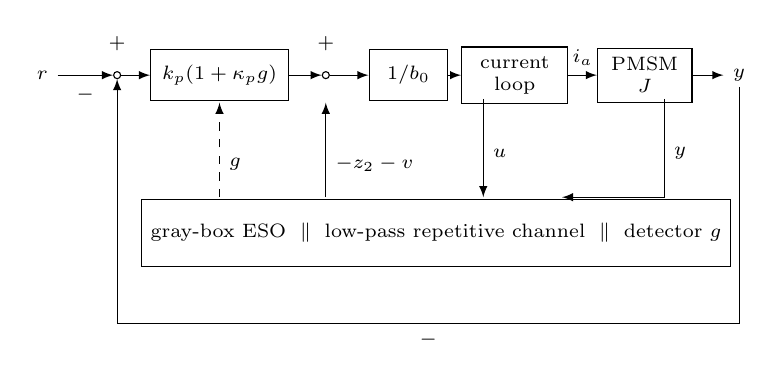
\begin{tikzpicture}[>=latex,font=\scriptsize,x=1cm,y=1cm]
\node (r) at (0,0) {$r$};
\node[draw,circle,inner sep=0.9pt] (s1) at (0.95,0) {};
\node[draw,minimum width=1.75cm,minimum height=0.65cm] (kp) at (2.25,0) {$k_p(1+\kappa_p g)$};
\node[draw,circle,inner sep=0.9pt] (s2) at (3.6,0) {};
\node[draw,minimum width=1.0cm,minimum height=0.65cm] (ib) at (4.65,0) {$1/b_0$};
\node[draw,minimum width=1.35cm,minimum height=0.65cm,align=center] (cl) at (6.0,0) {current\\loop};
\node[draw,minimum width=1.2cm,minimum height=0.65cm,align=center] (pl) at (7.65,0) {PMSM\\$J$};
\node (y) at (8.85,0) {$y$};
\node[draw,minimum width=5.8cm,minimum height=0.85cm,align=center] (ad) at (5.0,-2.0)
  {gray-box ESO \;$\|$\; low-pass repetitive channel \;$\|$\; detector $g$};
\draw[->] (r)--(s1);
\draw[->] (s1)--(kp);
\draw[->] (kp)--(s2);
\draw[->] (s2)--(ib);
\draw[->] (ib)--(cl);
\draw[->] (cl)-- node[above]{$i_a$} (pl);
\draw[->] (pl)--(y);
\draw (8.85,-0.15) -- (8.85,-3.15) -- (0.95,-3.15) -- (0.95,-0.15);
\draw[->] (0.95,-0.3) -- (0.95,-0.05);
\node[below] at (4.9,-3.15) {$-$};
\draw[->] (7.9,-0.3) -- (7.9,-1.55) node[pos=0.55,right]{$y$} -- (6.6,-1.55);
\draw[->] (5.6,-0.3) -- (5.6,-1.55) node[pos=0.55,right]{$u$};
\draw[->] (3.6,-1.55) -- (3.6,-0.35) node[pos=0.35,right]{$-z_2-v$};
\draw[->,dashed] (2.25,-1.55) -- (2.25,-0.35) node[pos=0.35,right]{$g$};
\node[above] at (0.95,0.18) {$+$};
\node[left] at (0.78,-0.25) {$-$};
\node[above] at (3.6,0.18) {$+$};
\end{tikzpicture}}
\caption{Signal flow of the proposed RCESO. The periodic component is reconstructed by
the low-pass repetitive channel and cancelled before the observer, so the ESO estimates
only the residual. The detector $g$ indexes the proportional gain (Law~D); the reset
operator of Law~F acts on $v$ and on the delay buffer only.}
\label{fig:block}
\end{figure}

\section{Adaptive Laws}\label{sec:laws}

\subsection{Law D: proportional-gain scheduling}\label{sec:lawd}
The load step is a non-periodic event, whereas the misalignment is periodic. This
difference is exploited by defining
\begin{equation}
g(t)=\frac{\bar e_1^2}{\bar e_1^2+\varepsilon_g^2},\qquad
\bar e_1(t)=\frac{1}{T}\int_{t-T}^{t}e_1(\sigma)\,\mathrm d\sigma ,
\label{eq:det}
\end{equation}
and scheduling the proportional gain as
\begin{equation}
k_p^{\rm eff}(t)=k_p\big[1+\kappa_p\,g(t)\big].
\label{eq:lawd}
\end{equation}
Any $k\cdot f_0$ component averages to zero over one full period, so $g$ is
\emph{structurally blind} to the periodic part of the fault and responds to the
non-periodic part only. No extra sensor, no load observer and no fault model are
needed: the detector is computed from $e_1$, which the control law already uses.
During a load step $g$ rises to $0.355$ on average (peak $0.954$, i.e., an equivalent
$k_p$ of $50$); at standstill it stays at $0.0000$ (peak $0.0003$), so the noise floor
is untouched, which is precisely where Law~B fails (Section~\ref{sec:results}).
Note that the 5.9~Hz cluster is not on the $1/T$ grid either, so $g$ also responds to
it ($0.100$--$0.111$ in the sustained segment); this is stated explicitly rather than
hidden, and it explains the sustained-segment improvement in Table~\ref{tab:lawd}.

\subsection{Law F: event-triggered state reset}\label{sec:lawf}
Law~D acts on the gain; the echo of \eqref{eq:echo} is a state problem. Law~F
therefore adds a reset operator applied only at the trigger instant:
\begin{equation}
\mathcal R_\alpha:\;\; v(t_{\rm trig}^+)=\alpha\,v(t_{\rm trig}^-),\qquad
v(t-T)\leftarrow\alpha\,v(t-T),
\label{eq:reset}
\end{equation}
with $\alpha=0$ for a withdrawal (clear) and $\alpha=-1$ for a reversal. The trigger
instant is
\begin{equation}
t_{\rm trig}=t_e+\tau,\qquad
\tau=\begin{cases}\tau_A\approx0, & \text{F-A}\\[0.6mm]
\tau_{\rm det}+\tau_{\rm dec}, & \text{F-B}\end{cases}
\label{eq:trig}
\end{equation}
where $\tau_{\rm det}\approx4\tau_f$ is the rise time of the fast envelope and
$\tau_{\rm dec}=N\Delta t$ the decision window. F-B obtains $t_e$ from a two-time-scale
envelope comparator,
\begin{equation}
\begin{aligned}
\dot E_f&=\frac{|e_1|-E_f}{\tau_f},\qquad \dot E_s=\frac{|e_1|-E_s}{\tau_s},\\
&\text{trigger}\iff E_f>k\,E_s ,
\end{aligned}
\label{eq:envelope}
\end{equation}
with $\tau_f=4$~ms, $\tau_s=500$~ms, $k=1.8$ and a cooldown of $0.3$~s.

\section{Stability}\label{sec:stab}
\subsection{Uniform ultimate boundedness of the nominal loop}
\begin{lemma}[repetitive channel]\label{lem:v}
For $|\st|\le1$ and $Q_0\in(0,1)$ the delay loop satisfies
\begin{equation}
\limsup_{t\to\infty}|v(t)|\le\bar v:=\frac{\beta_3}{1-Q_0}.
\label{eq:uubv}
\end{equation}
\end{lemma}
\begin{proof}
The input of the first-order lag is bounded by $Q_0\bar V+\beta_3$ with
$\bar V=\sup_{[t-T,t]}|v|$; iterating period by period and using
$|v(t)|\le W+(|v(0)|-W)e^{-t/\tau_0}$ yields the claim.
\end{proof}
The bound \eqref{eq:uubv} does not involve $e_1$: the $v$ channel is self-sustaining
and does not close an algebraic loop.

\begin{lemma}[observer error]\label{lem:eso}
Let the extended state satisfy $|\dot x_2|\le H$ and let $e_1=x_1-z_1$,
$e_2=x_2-z_2$. In scaled coordinates $\xi=[e_1,\;e_2/\omega_o]^{\!\top}$,
\begin{equation}
\dot\xi=\omega_o A_0\,\xi+w_d,\quad
A_0=\begin{bmatrix}-2&1\\-1&0\end{bmatrix},\quad
w_d=[-v,\;H/\omega_o]^{\!\top},
\label{eq:esiso}
\end{equation}
the Lyapunov equation $A_0^{\!\top}P_0+P_0A_0=-I$ is solved by
$P_0=\begin{bmatrix}0.5&-0.5\\-0.5&1.5\end{bmatrix}\succ0$, giving
\begin{equation}
\limsup_{t\to\infty}\|\xi(t)\|\le\frac{2\sqrt3}{\omega_o}
\sqrt{\bar v^{2}+\big(H/\omega_o\big)^{2}} .
\label{eq:uubeso}
\end{equation}
\end{lemma}

\begin{lemma}[tracking error]\label{lem:track}
With $\sigma=r-y$ and $\dot y=(b/b_0)(k_p\sigma-z_2-v)+d$,
\begin{equation}
\limsup_{t\to\infty}|\sigma(t)|\le\frac{b_0}{bk_p}
\Big(\sup|d|+\frac{b}{b_0}\big(\sup|x_2|+\bar v\big)\Big).
\label{eq:uubtrack}
\end{equation}
\end{lemma}

\begin{theorem}\label{thm:uub}
Under $|h|\le H$, positivity of $b,b_0,k_p,\omega_o,\tau_0,\zeta$, $Q_0\in(0,1)$ and
$\beta_3\ge0$, the nominal closed loop is UUB with the explicit bounds
\eqref{eq:uubv}--\eqref{eq:uubtrack}.
\end{theorem}

\subsection{Scheduling and reset do not enlarge the bound}
\begin{corollary}\label{cor:schedule}
With $g\in[0,1)$, $\kappa_p,\kappa_B\ge0$, the effective gains satisfy
$k_p^{\rm eff}\ge k_p$ and $\omega_o^{\rm eff}\ge\omega_o$; both right-hand sides of
\eqref{eq:uubeso} and \eqref{eq:uubtrack} are non-increasing in
$(\omega_o,k_p)$. Hence the nominal bound is also a bound of the scheduled loop:
scheduling does not enlarge the ultimate bound.
\end{corollary}
\begin{proposition}\label{prop:reset}
The reset operator \eqref{eq:reset} with $|\alpha|\le1$ preserves the UUB property.
\end{proposition}
\begin{proof}
Take $V=\tfrac12 v^2$. By \eqref{eq:reset}, $V(t_{\rm trig}^+)=\alpha^2V(t_{\rm trig}^-)
\le V(t_{\rm trig}^-)$, so the reset is a beneficial jump and does not invalidate
Theorem~\ref{thm:uub}; the price is one period of internal-model rebuilding, measured
as $+4.3\%$ in the steady-state window with a $0.3$~s cooldown.
\end{proof}

\begin{remark}
The bounds are conservative by two to five orders of magnitude compared with the
measured $|v|$ and $|e_1|$; their role is to establish structure (self-sustaining
channel, monotonicity in the gains), not to predict numbers. The quantitative behavior
is established numerically in Section~\ref{sec:results}.
\end{remark}

\section{Results}\label{sec:results}

\subsection{Numerical setup}
Table~\ref{tab:param} lists the parameters. Unless stated otherwise the drive runs at
600~rpm, the current loop at $f_{ci}=1$~kHz, the integration step is $10~\mu$s and the
trajectory is 12~s long. Random seeds are fixed so that every configuration sees the
same noise realization. The seven evaluation windows are those of
Table~\ref{tab:scenario}.

\begin{table}[!t]
\centering
\caption{Drive and controller parameters (simulation; bench values to be identified)}
\label{tab:param}
\footnotesize
\setlength{\tabcolsep}{3pt}
\begin{tabular}{@{}lll@{}}
\toprule
Quantity & Symbol & Value\\
\midrule
Rated torque / speed & $T_{\rm rated}$ / $n_{\rm rated}$ & 0.637~N$\cdot$m / 3000~rpm\\
Operating speed & $\omega_{\rm ref}$ & 600~rpm $=62.83$~rad/s\\
Torque constant / poles & $k_t$ / $p$ & 0.101~N$\cdot$m/A / 4\\
Inertia & $J$ & $1.89\times10^{-5}$~kg$\cdot$m$^2$\\
Line resistance / inductance & $R$ / $L$ & $0.35~\Omega$ / 1.14~mH\\
Per-unit gain / nominal & $b$ / $b_0$ & 536.41 / 643.69~s$^{-1}$\\
Speed-loop gain & $k_p$ & 75.36\\
Observer bandwidth & $\omega_o$ & 500~rad/s\\
Repetitive gain / constant & $\beta_3$ / $\tau_0$ & 2000 / 5~ms\\
Forgetting factor & $Q_0$ & 0.98\\
Saturation & $\zeta$ & 0.2\\
Current-loop bandwidth & $f_{ci}$ & 1~kHz\\
Integration step & $\Delta t$ & $10~\mu$s\\
Current noise & $\sigma_i$ & 1\% rated (0.063~A)\\
Load noise & $\sigma_T$ & 5\% rated (0.0319~N$\cdot$m)\\
\bottomrule
\end{tabular}
\end{table}

\subsection{Why the repetitive channel is necessary}
Table~\ref{tab:algo} and Fig.~\ref{fig:pieso} compare four structures on the same
light-load condition ($\pm0.12$~N$\cdot$m). PI and pure ESO both lack a periodic
internal model; their steady-state errors are 311.15 and 82.85~rpm, i.e., 10.6 and 2.8
times the 29.24~rpm of the RCESO. Adding Law~D buys the load transient
(56.69~$\to$~39.87~rpm, $1.42\times$) rather than the steady state
(29.24~$\to$~28.41~rpm, $-2.8\%$), which is the first indication that the two
mechanisms act on different windows.

\begin{table}[!t]
\centering
\caption{Four-structure comparison on the light-load condition (speed-error RMS in rpm; the peak current is 5.20--5.21~A in all four cases)}
\label{tab:algo}
\scriptsize
\setlength{\tabcolsep}{2.2pt}
\begin{tabular}{@{}lrrrrrrr@{}}
\toprule
Structure & no-load & step & ev.1 & ev.2 & post & sust. & steady\\
\midrule
PI ($k_i=400$) & 52.51 & 1167.50 & 378.45 & 295.30 & 249.20 & 313.93 & 311.15\\
ESO           & 29.50 & 107.67 & 83.83 & 76.08 & 57.80 & 83.90 & 82.85\\
RCESO         & 13.56 & 56.69 & 27.50 & 29.90 & 29.67 & 28.88 & 29.24\\
RCESO+Law D   & 13.55 & 39.87 & 27.31 & 29.04 & 28.72 & 28.11 & 28.41\\
\bottomrule
\end{tabular}
\end{table}

\begin{figure*}[!t]
\centering
\includegraphics[width=0.85\textwidth]{fig_pi_eso.pdf}
\caption{Structures without an internal model (PI, pure ESO) versus those with one.
(a) Time domain (100~ms envelope plus mean). (b) Seven-window RMS on a logarithmic
axis. The failure of PI and ESO is structural (no $k\cdot f_0$ internal model), not a
matter of tuning; scaling the load amplitude scales the errors but leaves the ratios
unchanged.}
\label{fig:pieso}
\end{figure*}

\subsection{Law D and the $2^2$ ablation over Laws B and D}
Table~\ref{tab:lawd} isolates Law~D under the $A=0.30$ condition: every one of the
seven windows improves simultaneously (Pareto improvement), the load transient from
66.80 to 48.36~rpm ($-27.6\%$), with the peak current unchanged at 6.77~A.
Table~\ref{tab:ablation} expands this into a $2^2$ full-factorial experiment over the
two candidate schedules (Law~B, Law~D).

\begin{table}[!t]
\centering
\caption{Law D alone ($\kappa_p=4$, $\varepsilon_g=0.01$), speed-error RMS in rpm}
\label{tab:lawd}
\scriptsize
\setlength{\tabcolsep}{2.2pt}
\begin{tabular}{@{}lrrrrrrr@{}}
\toprule
Configuration & no-load & step & ev.1 & ev.2 & post & sust. & steady\\
\midrule
baseline & 13.56 & 66.80 & 63.00 & 50.20 & 49.71 & 52.30 & 52.45\\
Law D    & 13.55 & $\mathbf{48.36}$ & $\mathbf{59.58}$ & $\mathbf{46.48}$ & $\mathbf{43.74}$ & $\mathbf{48.11}$ & $\mathbf{47.97}$\\
change   & $0.0\%$ & $\mathbf{-27.6\%}$ & $-5.4\%$ & $-7.4\%$ & $-12.0\%$ & $-8.0\%$ & $-8.5\%$\\
\bottomrule
\end{tabular}
\end{table}

\begin{table*}[!t]
\centering
\caption{$2^2$ full-factorial ablation over $(B,D)$; speed-error RMS in rpm}
\label{tab:ablation}
\footnotesize
\setlength{\tabcolsep}{4pt}
\begin{tabular}{@{}lrrrrrrrr@{}}
\toprule
$(B,D)$ & no-load & step & ev.1 & ev.2 & post & sust. & steady & $\max|i_a|$ (A)\\
\midrule
(0,0) baseline    & 13.56 & 66.80 & 63.00 & 50.21 & 49.71 & 52.30 & 52.45 & 6.77\\
(0,1) Law D only  & 13.55 & $\mathbf{48.36}$ & $\mathbf{59.58}$ & $\mathbf{46.48}$ & $\mathbf{43.74}$ & $\mathbf{48.11}$ & $\mathbf{47.97}$ & 6.77\\
(1,0) Law B only  & 13.55 & 61.72 & 65.54 & 51.00 & 47.86 & 53.71 & 53.17 & 6.75\\
(1,1) B$+$D       & 13.55 & 48.59 & 61.61 & 47.56 & 43.26 & 49.71 & 49.08 & 6.75\\
\midrule
\multicolumn{9}{@{}l}{\emph{main effects} (1 minus 0; negative is better)}\\
Law B & $-0.00$ & $-2.42$ & $+2.29$ & $+0.94$ & $-1.17$ & $+1.51$ & $+0.92$ & \\
Law D & $+0.00$ & $\mathbf{-15.79}$ & $\mathbf{-3.68}$ & $\mathbf{-3.58}$ & $\mathbf{-5.28}$ & $\mathbf{-4.10}$ & $\mathbf{-4.29}$ & \\
\bottomrule
\end{tabular}
\end{table*}

Three observations follow. (i) Law~D has a negative main effect in every window and is
the only factor with a Pareto improvement; (ii) Law~B helps only the load step
($-2.42$~rpm) and degrades event~1 ($+2.29$), the sustained segment ($+1.51$) and the
steady state ($+0.92$): raising $\omega_o$ injects current noise into $z_2$, which this
drive cannot absorb; (iii) the interaction $B\times D$ is positive in six of the seven
windows---up to $+5.32$~rpm on the load step---so the two schedules fight each other
on exactly the window where Law~B is supposed to help. The recommended configuration
is therefore the baseline plus Law~D, without stacking Law~B.
Fig.~\ref{fig:ablation} shows the four groups, the main effects and their interaction.

\begin{figure*}[!t]
\centering
\includegraphics[width=0.95\textwidth]{fig_ablation_2x2.pdf}
\caption{$2^2$ ablation over Laws~B and~D: (a) per-window RMS of the four groups;
(b) main effects and the $B\times D$ interaction. Law~D is negative in all seven
windows; Law~B reduces only the load transient and degrades the others; the two
schedules are antagonistic on the load step.}
\label{fig:ablation}
\end{figure*}

\subsection{Echo suppression with Law F}
Table~\ref{tab:echo} quantifies the two implementations on the withdrawal and
reversal events. F-A, which uses an external event signal, suppresses the first-cycle
10~Hz echo by $74.5\%$ at a $0.2\%$ steady-state cost; F-B, which has to detect the
event from the speed error, reaches the trigger about $40$~ms late and retains only
$-30.4\%$ of the achievable suppression, at $+4.3\%$ steady-state cost. This is the
direct confirmation of the timing law \eqref{eq:timing}: the mechanism is not limited
by how hard the state is reset but by how accurately the event instant is known.
Fig.~\ref{fig:echoab} shows the corresponding timing; the steady-state cost of the
two operating points is the last row of Table~\ref{tab:echo}.

\begin{table}[!t]
\centering
\caption{Echo suppression: first-cycle 10~Hz component (rpm) and steady-state cost}
\label{tab:echo}
\footnotesize
\setlength{\tabcolsep}{3pt}
\begin{tabular}{@{}lccc@{}}
\toprule
Case & no reset & F-B (40~ms) & F-A (event)\\
\midrule
withdrawal, 1st cycle & 127.7 & 88.9 ($-30.4\%$) & $\mathbf{32.5}$ ($-74.5\%$)\\
reversal, 1st cycle   & 253.8 & 159.8 ($-37.0\%$) & $\mathbf{142.5}$ ($-43.9\%$)\\
steady-state 10~Hz    & 46.7 & 48.7 & 46.8\\
cost in steady window & --- & $+4.3\%$ & $+0.2\%$\\
\bottomrule
\end{tabular}
\end{table}

\PH{Fig.~\ref{fig:expecho}: measured echo after the withdrawal event, F-A versus F-B,
to be compared with Fig.~\ref{fig:echoab}. The event instant must be time-stamped in
the same clock as the controller; otherwise $\tau$ of \eqref{eq:timing} cannot be
verified.}
\begin{figure}[!t]
\centering
\fbox{\parbox[c][3.6cm][c]{0.94\columnwidth}{\centering\color{red!70!black}\footnotesize
\textbf{[TO BE FILLED]}\\[2mm]
Measured first-cycle echo after the withdrawal event (F-A, F-B, no reset) and the
corresponding per-cycle 10~Hz amplitude.}}
\caption{Measured echo [TO BE FILLED].}
\label{fig:expecho}
\end{figure}


\begin{figure*}[!t]
\centering
\includegraphics[width=0.86\textwidth]{fig_echo_ab.pdf}
\caption{Timing comparison of F-A and F-B on the withdrawal case, all other conditions
equal. (a) Speed error after the event: F-A resets at the event instant, F-B about
$40$~ms later; the difference is exactly the $\tau$ of \eqref{eq:timing}.
(b) Per-cycle 10~Hz amplitude: 32.5 (F-A) and 88.9 (F-B) against 127.7~rpm with no
reset.}
\label{fig:echoab}
\end{figure*}



\subsection{Sensitivity}
Fig.~\ref{fig:b0} shows the effect of the nominal-gain mismatch. Speed error decreases
monotonically as $b_0/b$ decreases ($87.60$~rpm at $b_0/b=2$, $52.45$ at the design
value $1.2$, $23.25$ at $0.5$), at the price of a $6.7\%$ current increase
($6.77\to7.22$~A). The design value with a $20\%$ margin is thus conservative on this
object; values below $0.5$ were not tested and no stability claim is made for them.
Fig.~\ref{fig:fft} provides the frequency-domain evidence: the internal model reduces
the 10/30/50~Hz components by $8.8/7.5/5.6$ times while leaving the off-grid 5.9~Hz
cluster almost untouched, as the internal-model principle predicts.

\begin{figure}[!t]
\centering
\includegraphics[width=0.95\columnwidth]{fig_b0.pdf}
\caption{Effect of $b_0$ mismatch. Speed error is monotone in $b_0/b$; the nominal
value with a $20\%$ margin is conservative here, but its stability margin and smaller
values were not evaluated.}
\label{fig:b0}
\end{figure}

\begin{figure*}[!t]
\centering
\includegraphics[width=0.82\textwidth]{fig_fft.pdf}
\caption{Frequency-domain comparison in the steady-state window (7--12~s, Hann
window). (a) Disturbance spectrum: 5.9~Hz cluster and misalignment harmonics.
(b) Speed-error spectra. (c) Peak comparison: 10, 30 and 50~Hz are suppressed by
8.8, 7.5 and 5.6 times, whereas 5.9~Hz is essentially unchanged.}
\label{fig:fft}
\end{figure*}

\subsection{Experimental validation (to be completed)}
The bench is the drive used for the per-unit model: motor SM060R20C30M0AD, drive
DM807, 2500~PPR encoder, programmable load machine, torque transducer and a
data-acquisition channel synchronized to the PWM carrier. The controller runs at
[TO BE FILLED] kHz, which is intentionally below the $10~\mu$s step of the simulation;
the resulting degradation must be measured, not extrapolated.

\PH{Fig.~\ref{fig:bench}: photograph of the test bench with the motor--coupling--load
train, the torque transducer and the drive cabinet labelled. Replace this box with the
photograph.}
\begin{figure*}[!t]
\centering
\fbox{\parbox[c][4.0cm][c]{0.9\textwidth}{\centering\color{red!70!black}\footnotesize
\textbf{[TO BE FILLED]}\\[2mm]
Bench photograph: motor SM060R20C30M0AD $\rightarrow$ coupling (misalignment shim)
$\rightarrow$ torque transducer $\rightarrow$ load machine; drive DM807 and the
control board are to be labelled.}}
\caption{Experimental setup [TO BE FILLED].}
\label{fig:bench}
\end{figure*}

\PH{Table~\ref{tab:bench}: measured window RMS for PI, ESO, RCESO, RCESO+Law~D and
RCESO+Law~F(A/B) on the bench, same seven windows as Table~\ref{tab:ablation}.}
\begin{table}[!t]
\centering
\caption{Measured window RMS (rpm) on the test bench [TO BE FILLED]}
\label{tab:bench}
\footnotesize
\setlength{\tabcolsep}{3pt}
\begin{tabular}{@{}lrrrrrrr@{}}
\toprule
Configuration & no-load & step & ev.1 & ev.2 & post & sust. & steady\\
\midrule
PI            & --- & --- & --- & --- & --- & --- & ---\\
ESO           & --- & --- & --- & --- & --- & --- & ---\\
RCESO         & --- & --- & --- & --- & --- & --- & ---\\
RCESO+Law D   & --- & --- & --- & --- & --- & --- & ---\\
RCESO+Law F-B & --- & --- & --- & --- & --- & --- & ---\\
RCESO+Law F-A & --- & --- & --- & --- & --- & --- & ---\\
\bottomrule
\end{tabular}
\end{table}

\PH{Fig.~\ref{fig:expspeed}: measured speed error for the five configurations, same
axes and windows as Fig.~\ref{fig:ablation}(a). Use the 100~ms envelope plus mean so
that the 10~Hz component is visible; annotate the load-step dip in rpm.}
\begin{figure*}[!t]
\centering
\fbox{\parbox[c][3.9cm][c]{0.9\textwidth}{\centering\color{red!70!black}\footnotesize
\textbf{[TO BE FILLED]}\\[2mm]
Measured speed error (rpm) versus time for PI / ESO / RCESO / RCESO+Law~D /
RCESO+Law~F, plus the load-step zoom. Export from the DAQ at the speed-loop rate,
not at the PWM rate.}}
\caption{Measured speed error [TO BE FILLED].}
\label{fig:expspeed}
\end{figure*}



\PH{Computation cost: measure the execution time of the ESO, the repetitive channel,
Law~D and Law~F on the target controller (percent of the [TO BE FILLED]~$\mu$s
speed-loop budget). This is a standard reviewer request for TIE/TTE and must not be
estimated.}

\section{Conclusion}\label{sec:concl}
This paper has shown that the two dominant weaknesses of a repetitive-control-enhanced
ESO on a low-inertia PMSM drive have different natures and therefore need different
remedies. The load-step dip is an information problem: the $T$-window mean of the
tracking error is blind to the periodic fault and reacts to non-periodic events, so
scheduling the proportional gain with it (Law~D) improves all seven evaluation windows
at once, with a $27.6\%$ reduction of the transient error and no penalty in peak
current. The echo is a state problem: once the disturbance pattern changes, the delay
line keeps replaying the old memory for a full period, and the pump term is too fast
for any parameter change to track it; the correction must therefore act on the state.
An event-triggered reset does exactly that, and its achievable suppression is bounded
by the accuracy with which the event instant is known ($74.5\%$ with a feedforward
signal, $30.4\%$ with an envelope detector).
The UUB analysis covers both mechanisms: the repetitive channel is self-sustaining,
scheduling does not enlarge the ultimate bound, and the reset is a beneficial jump.
Future work includes closing the detection loop with a low-latency observer, extending
the analysis to random noise, and completing the experimental campaign
[TO BE FILLED].

\section*{Acknowledgment}
The authors thank [TO BE FILLED] for the test-bench access and [TO BE FILLED] for
discussions on the echo mechanism.

\IEEEtriggeratref{12}

\begin{thebibliography}{18}
\bibitem{nandi2005}
S.~Nandi, H.~A. Toliyat, and X.~Li, \qq{Condition monitoring and fault diagnosis of
electrical motors---A review}, \emph{IEEE Trans. Energy Convers.}, vol.~20, no.~4,
pp.~719--729, Dec. 2005.

\bibitem{han2009}
J.~Han, \qq{From PID to active disturbance rejection control}, \emph{IEEE Trans. Ind.
Electron.}, vol.~56, no.~3, pp.~900--906, Mar. 2009.

\bibitem{gao2003}
Z.~Gao, \qq{Scaling and bandwidth-parameterization based controller tuning}, in
\emph{Proc. Amer. Control Conf.}, 2003, pp.~4989--4996.

\bibitem{inoue1981}
T.~Inoue, M.~Nakano, and S.~Iwai, \qq{High accuracy control of a proton synchrotron
magnet power supply}, in \emph{Proc. IFAC World Congr.}, 1981, pp.~3137--3142.

\bibitem{hara1988}
S.~Hara, Y.~Yamamoto, T.~Omata, and M.~Nakano, \qq{Repetitive control system: A new
type servo system for periodic exogenous signals}, \emph{IEEE Trans. Autom. Control},
vol.~33, no.~7, pp.~659--668, Jul. 1988.

\bibitem{tomizuka1988}
M.~Tomizuka, T.-C. Tsao, and K.-K. Chew, \qq{Discrete-time domain analysis and
synthesis of repetitive controllers}, in \emph{Proc. Amer. Control Conf.}, 1988,
pp.~860--866.

\bibitem{longman2000}
R.~W. Longman, \qq{Iterative learning control and repetitive control for engineering
practice}, \emph{Int. J. Control}, vol.~73, no.~10, pp.~930--954, Jul. 2000.

\bibitem{francis1976}
B.~A. Francis and W.~M. Wonham, \qq{The internal model principle of control theory},
\emph{Automatica}, vol.~12, no.~5, pp.~457--465, Sep. 1976.

\bibitem{zhou2001}
K.~Zhou and D.~Wang, \qq{Digital repetitive learning controller for three-phase CVCF
PWM inverter}, \emph{IEEE Trans. Ind. Electron.}, vol.~48, no.~4, pp.~820--830,
Aug. 2001.

\bibitem{chen2016}
W.-H. Chen, J.~Yang, L.~Guo, and S.~Li, \qq{Disturbance-observer-based control and
related methods---An overview}, \emph{IEEE Trans. Ind. Electron.}, vol.~63, no.~2,
pp.~1083--1095, Feb. 2016.

\bibitem{sul2011}
S.-K. Sul, \emph{Control of Electric Machine Drive Systems}. Hoboken, NJ, USA:
Wiley-IEEE Press, 2011.

\bibitem{leonhard2001}
W.~Leonhard, \emph{Control of Electrical Drives}, 3rd ed. Berlin, Germany: Springer,
2001.

\bibitem{khalil2002}
H.~K. Khalil, \emph{Nonlinear Systems}, 3rd ed. Upper Saddle River, NJ, USA:
Prentice Hall, 2002.

\bibitem{bodson2005}
M.~Bodson, \qq{Rejection of periodic disturbances of unknown and time-varying
frequency}, \emph{Int. J. Adapt. Control Signal Process.}, vol.~19, no.~2--3,
pp.~67--88, 2005.

\bibitem{chew1990}
K.~K. Chew and M.~Tomizuka, \qq{Digital control of repetitive errors in disk drive
systems}, \emph{IEEE Control Syst. Mag.}, vol.~10, no.~1, pp.~16--20, Jan. 1990.

\bibitem{krause2002}
P.~C. Krause, O.~Wasynczuk, and S.~D. Sudhoff, \emph{Analysis of Electric Machinery
and Drive Systems}, 2nd ed. Piscataway, NJ, USA: IEEE Press, 2002.

\bibitem{schoen1995}
R.~R. Schoen, B.~K. Lin, T.~G. Habetler, J.~H. Schlag, and S.~Farag,
\qq{An unsupervised, on-line system for induction motor fault detection using stator
current monitoring}, \emph{IEEE Trans. Ind. Appl.}, vol.~31, no.~6, pp.~1280--1286,
Nov./Dec. 1995.

\bibitem{gao2001}
Z.~Gao, Y.~Huang, and J.~Han, \qq{An alternative paradigm for control system design},
in \emph{Proc. IEEE Conf. Decis. Control}, 2001, pp.~4578--4585.
\end{thebibliography}

\end{document}
